\documentclass[12pt]{report}
\usepackage{amsmath}
\usepackage{graphicx}
\usepackage[colorlinks=true, linkcolor=black, citecolor=black, filecolor=black, urlcolor=black]{hyperref}
\usepackage{lipsum}
\usepackage{titlesec}
\usepackage{pdfpages}
\usepackage{float}
\usepackage[utf8]{inputenc}
\title{Heat Production Management Project for Semester Project 2}
\author{Kacper Grzyb \and Sebestyen Deak \and Ignad Bozhinov \and Leonardo Gianola \and Levente Sohar}
\date{03-06-2024}

% Define a command to convert number section counting to alphabetical section counting
\makeatletter
\newcommand{\alphsection}{\@alph\c@section}
\makeatother

% Redefine the sectioning commands
\renewcommand{\thesection}{\thechapter\alphsection}
\titleformat{\section}
  {\normalfont\Large\bfseries}{\thesection}{1em}{}


\begin{document}
\maketitle

\tableofcontents

% Chapter 1
\chapter{Introduction}
Introduction chapter goes here

% Chapter 2
\chapter{Release Planning}
Release Planning chapter goes here

% Chapter 3
\chapter{Sprint Materials}
In this chapter all the materials from the sprints can be found.




\section{Sprint 1}

\subsection{Retrospective}
\textbf{Project:} Semester Project Group 11 \\
\textbf{Sprint Duration:} March 5 - March 19, 2024 \\
\textbf{Team Members:} Levente Sohár, Ignat Bozhinov, Leonardo Gianola, Kacper Grzyb, Sebestyén Deák \\
\textbf{Stakeholders:} Sadok Ben Yahia

\subsection*{1. Sprint Goals and Outcomes}

\begin{itemize}
    \item \textbf{Goal 1:} Move epic and user stories into Jira\\
    \textbf{Status:} Completed. All the epics and user stories are in Jira now.
    \item \textbf{Goal 2:} Divide Roles\\
    \textbf{Status:} Completed. Product Owner and Scrum Master Roles have been given.
    \item \textbf{Goal 3:} Create .gitignore file\\
    \textbf{Status:} Completed. Created .gitignore file.
    \item \textbf{Goal 4:} Break down User Stories into requirements with MoSCoW\\
    \textbf{Status:} Completed. All the different User Stories have a Must Do (-M), Should Do (-S), Can Do (-C), Would Not Do (-W).
    \item \textbf{Goal 5:} Rewrite tasks into User Stories\\
    \textbf{Status:} Completed.
    \item \textbf{Goal 6:} Add User Points to User Stories\\
    \textbf{Status:} Completed. Every User Story has been rated in story points.
    \item \textbf{Goal 7:} Gantt Chart\\
    \textbf{Status:} Completed. Every Task has been estimated, and a Gantt Chart has been made according to this and our timeframe.
    \item \textbf{Goal 8:} Create Sprint Review\\
    \textbf{Status:} Completed.
\end{itemize}

\subsection*{2. Completed Work}
Transitioning our project management to Jira, we've streamlined our workflow and enhanced visibility into our tasks and progress. Recognizing the importance of role clarity in optimizing team performance, we successfully delineated roles and responsibilities. Implementing best practices in version control, we established a .gitignore file. Employing the MoSCoW method to prioritize requirements, we gained clarity on project scope and stakeholder expectations. Restructuring our tasks into user stories, we've shifted our focus from implementation details to user-centric outcomes, fostering a deeper understanding of user needs and motivations. Introducing user points to our user stories allowed us to quantify complexity and effort more accurately, facilitating resource allocation and sprint planning. Creating a Gantt chart provided us with a visual roadmap for project execution, enabling us to sequence tasks, allocate resources, and identify dependencies more effectively. Instituting sprint reviews has fostered transparency, accountability, and continuous improvement within our agile framework.
\subsection*{3. Unfinished Work}
Everything we set out to do during this sprint we have accomplished.
\subsection*{4. Quality and Technical Issues}
We haven't started coding yet, and only used already established software for our work, therefore we didn't have any technical issues.
\subsection*{5. Team Dynamics and Collaboration}
Work has been mostly divided equally, with everyone doing their part. Communication was clear and to the point.
\subsection*{6. Processes and Tools}
Jira helps keep track of the backlog and manage the sprint. For making the Gantt Chart, Canva was used, which helped speed up the process.
\subsection*{7. Stakeholder Feedback}
When talking with our supervisor Sadok, he approved of the direction we were heading this sprint, emphasizing making Dashboards.
\subsection*{8. Obstacles and Impediments}
We have been able to complete all the goals without any obstacles or impediments.
\subsection*{9. Successes and Wins}
The biggest win for the team was finishing all of our goals in time.
\subsection*{10. Action Items for Improvement}
Breaking the requirement into small tasks that can be worked on independently, therefore not everything has to be done in the one meeting we weekly.

\hfill 2024.03.16


\begin{figure}[H]
  \centering
  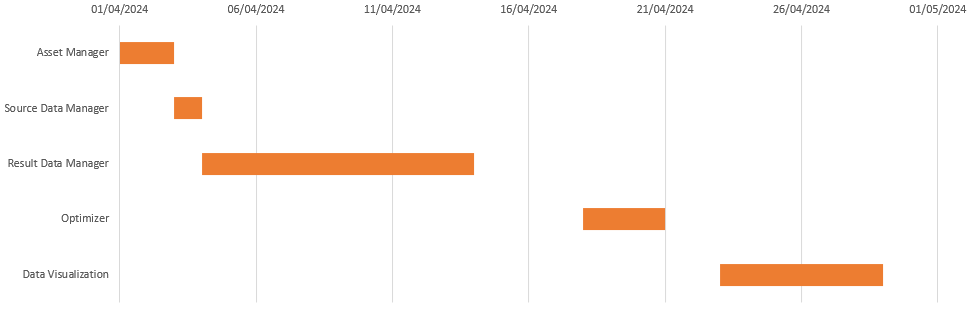
\includegraphics[width=1\textwidth]{Resources/1-Sprint/Gantt-Chart-Optimal.png}
  \caption{Optimal Gantt Chart}
  \label{fig:OptGanttChart-image}
\end{figure}

\begin{figure}[H]
  \centering
  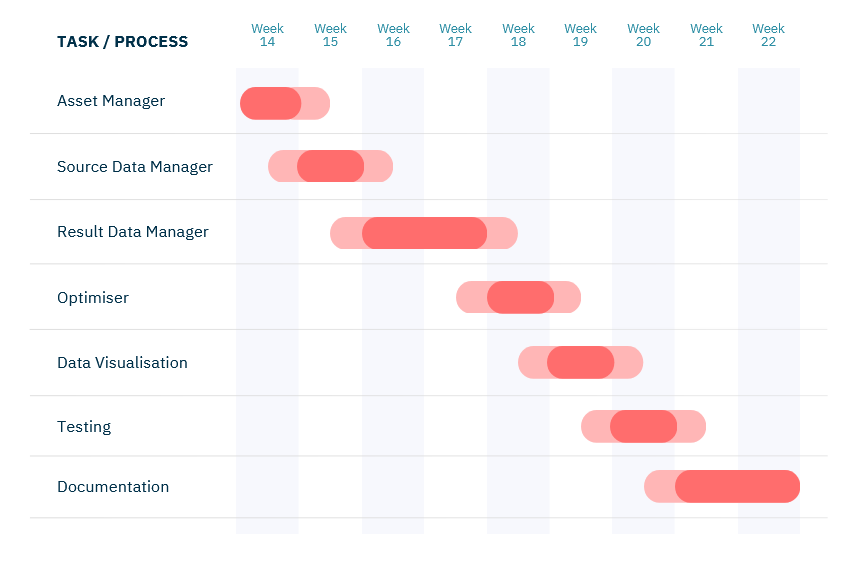
\includegraphics[width=1\textwidth]{Resources/1-Sprint/Gantt-Chart-Realistic.png}
  \caption{Realistic Gantt Chart}
  \label{fig:RealGanttChart-image}
\end{figure}




\section{Sprint 2}
%Planning
\subsection{Planning}
\begin{figure}[H]
  \centering
  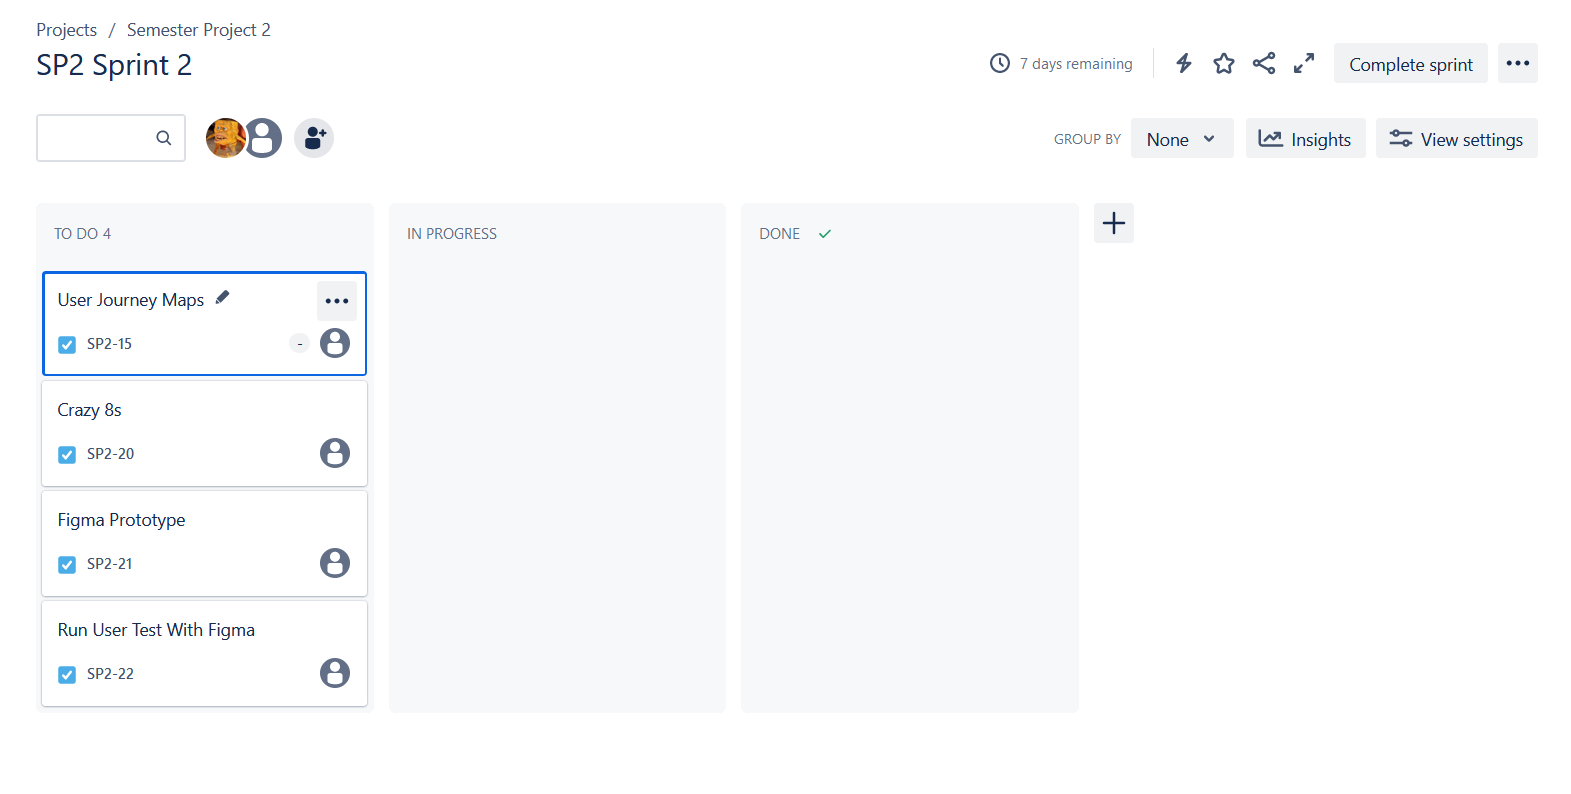
\includegraphics[width=1\textwidth]{Resources/2-Sprint/Planning/Sprint2_Planning_Package.png}
  \caption{Sprint 2 Planning Package}
  \label{fig:S2Planning-image}
\end{figure}

%Daily Scrum
\subsection*{Daily Scrum 02/04/2024}

\begin{itemize}
    \item The team completed 2 out of 4 issues.
    \item 2 issues are currently in progress, one of which is very close to being finished and the other one is expected to be finished by the end of the week.
\end{itemize}

\subsection*{Roadblocks}
\begin{itemize}
    \item The team faced a few conflicting ideas and a wrong understanding of how the Result Data Manager and Asset Manager components are supposed to look like. They were solved through an online Discord meeting.
    \item Some team members are still on holidays, which makes organising work a bit harder.
\end{itemize}

\subsection*{Plans for the rest of the Sprint}
\begin{itemize}
    \item Polish the Figma prototype made.
    \item Get feedback on the Figma prototype.
    \item Begin discussion about starting the development phase.
\end{itemize}

\subsection*{Metrics and Progress}
The team has attached screenshots of the current state of the sprint backlog and the sprint status report to give information about how much work has been done and how much work still needs to be done.

\begin{figure}[H]
  \centering
  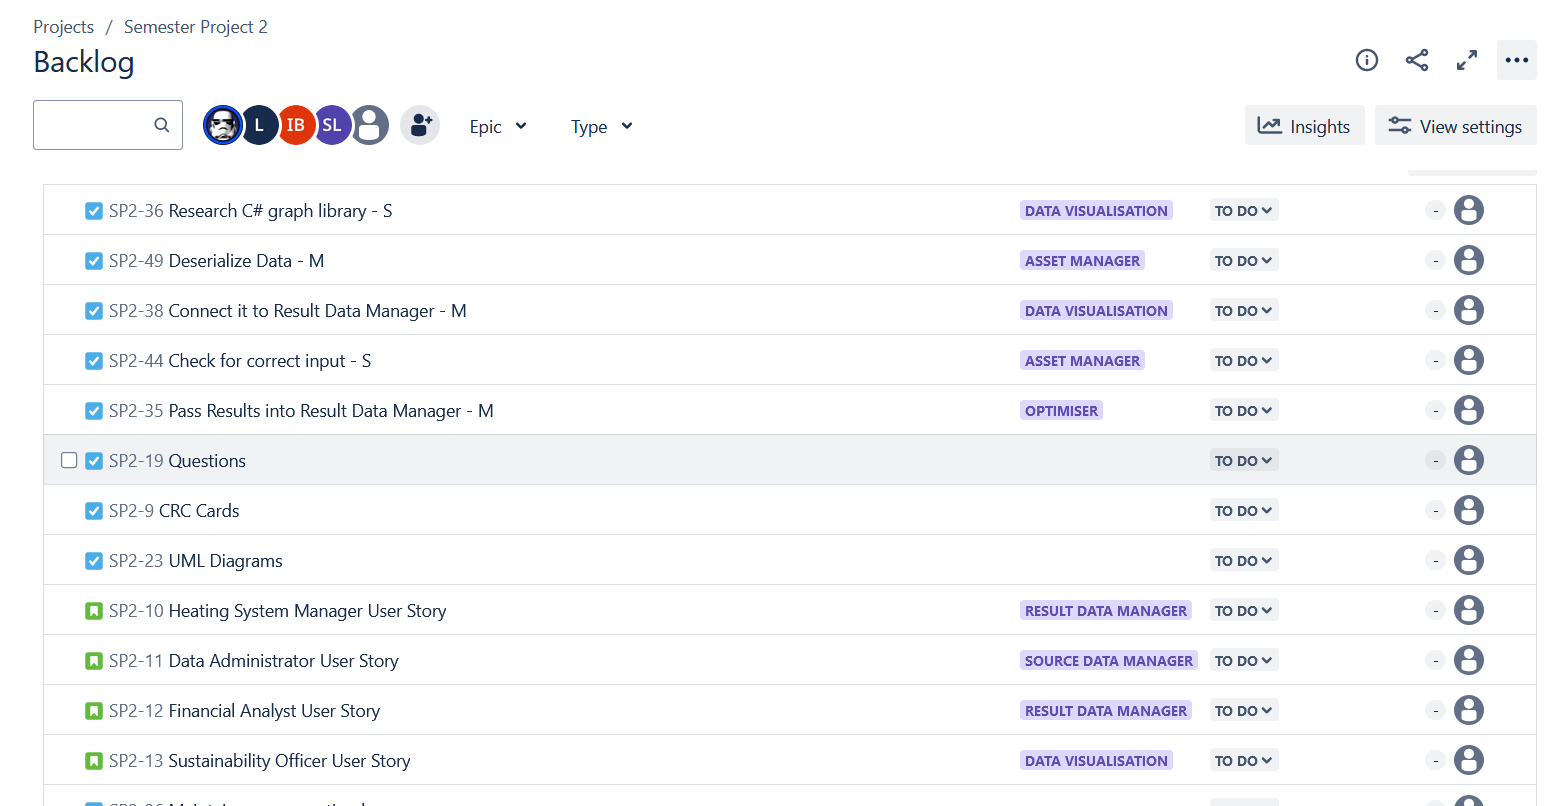
\includegraphics[width=1\textwidth]{Resources/2-Sprint/Daily-Scrum/backlog1.png}
  \caption{Daily Scrum Backlog 1}
  \label{fig:S2Scrum1-image}
\end{figure}

\begin{figure}[H]
  \centering
  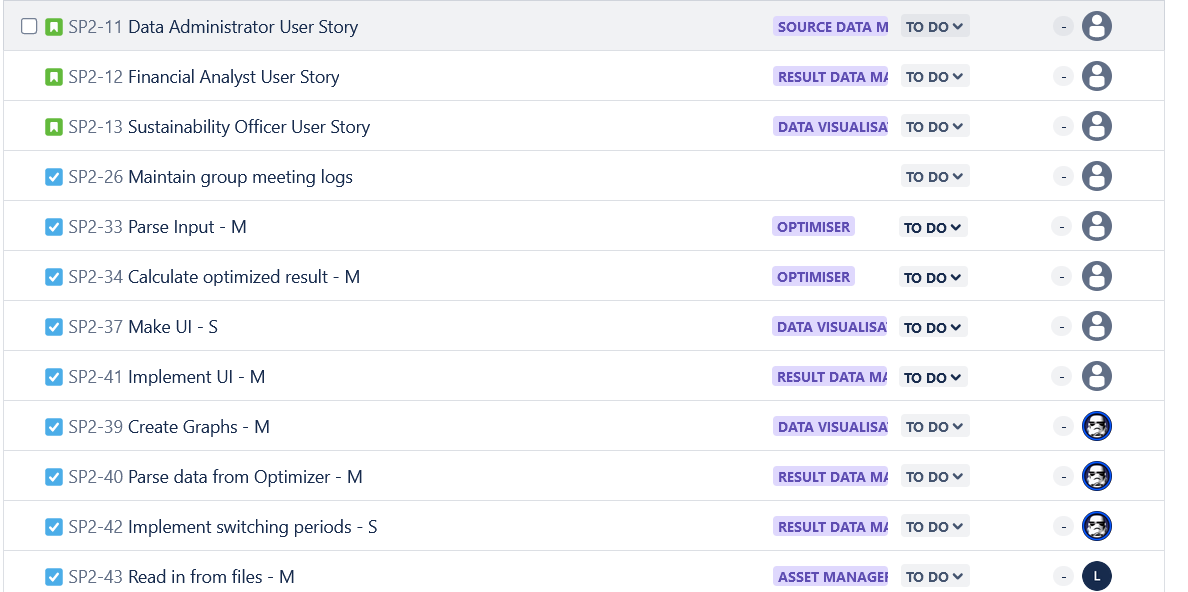
\includegraphics[width=1\textwidth]{Resources/2-Sprint/Daily-Scrum/backlog2.png}
  \caption{Daily Scrum Backlog 2}
  \label{fig:S2Scrum2-image}
\end{figure}

\begin{figure}[H]
  \centering
  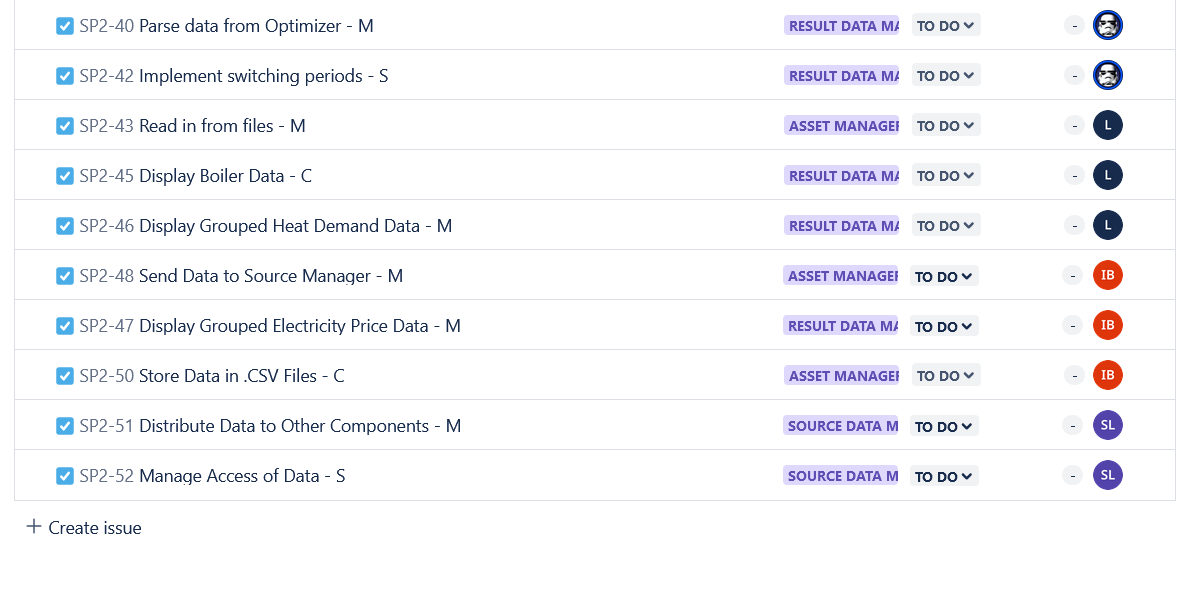
\includegraphics[width=1\textwidth]{Resources/2-Sprint/Daily-Scrum/backlog3.png}
  \caption{Daily Scrum Backlog 3}
  \label{fig:S2Scrum3-image}
\end{figure}

%Retrospect

\subsection*{Sprint 2 Retrospective}

\subsection*{What went well}
\begin{itemize}
    \item Remote meeting to re-align on the project direction
    \item All sprint tasks done despite remote work due to the Easter holidays
    \item Remote communication
    \item Willingness to pivot, make changes to the project
\end{itemize}

\subsection*{What to improve}
\begin{itemize}
    \item Spend more time on understanding the project requirements -- the team had a wrong idea of what the Result Data Manager, Asset Manager and Source Data Manager should consist of which created a setback and meant some of the plans for the project need to be remade, such as the tasks on Jira
    \item Pay attention to time zones when doing remote work -- the time zone difference created a minor issue during one of the team's remote meetings
    \item Plan out and divide work more carefully to avoid misunderstandings and vagueness
\end{itemize}

\subsection*{What the team aims to improve in the next Sprint}
\begin{itemize}
    \item Align the project with the requirements
    \item Remove vagueness from the project direction
    \item Remove vagueness from tasks for each team member
\end{itemize}


\section{Sprint 3}
\section{Sprint 4}


% Chapter 4
\chapter{Technical Details}
Technical Details Chapter goes here

% Chapter 4a
\section{Design and UML Diagrams}
Design and UML Diagrams yapping goes here

% Chapter 4b
\section{Simple Design}
Simple design yapping goes here

% Chapter 4c
\section{Incremental Design}
Incremental Design yapping goes here

% Chapter 4d
\section{Refactoring}
Refactoring yapping goes here

% Chapter 4e
\section{Test-Driven Development}
Test-Driven Development yapping goes here

% Chapter 4f
\section{Unit Testing}
Unit Testing yapping goes here

% Chapter 4g
\section{Pair Programming}
Pair Programming yapping goes here

% Chapter 4h
\section{Code Review}
Code Review yapping goes here

% Chapter 5
\chapter{Conclusion and Group's Reflections}
Conclusion chapter goes here

% Chapter 5a
\section{Working on a common project with other groups}
5a yapping goes here

% Chapter 5b
\section{What went well and not so well with the group's specific set of tasks}
5b yapping goes here

% Chapter 5c
\section{Specific contributions of each team member}
5c yapping goes here

\section{Future actions to prevent problems and difficulties faced during the project}
5d yapping goes here


\end{document}